\documentclass[10pt,a4paper]{article}
\usepackage[italian]{babel}
\usepackage[T1]{fontenc}
\usepackage[utf8]{inputenc}
\usepackage[affil-it]{authblk}
\usepackage{lineno,hyperref}
\usepackage{amsmath}
\usepackage{amsfonts}
\usepackage{amssymb}
\usepackage{graphicx}

\newtheorem{remark}{Osservazione}
\newtheorem{definition}{Definizione}
\newtheorem{theorem}{Teorema}

\newcommand{\ww}{\mathbf{w}}
\newcommand{\vv}{\mathbf{v}}
\newcommand{\ee}{\mathbf{e}}

\begin{document}
\title{Appunti di Artificial Intelligence}

\author{Ivan Masnari%
  \thanks{e-mail: \texttt{ivan.masnari@studenti.unimi.it}}}
\affil{Facoltà di Informatica, UniMi, Milano}

\date{Ultima modifica: \today}
\maketitle
\section{Introduzione}

Dato un qualunque sistema, se disponiamo di un insieme di leggi o regole che lo descrivono completamente (nel caso di un sistema fisico avremmo delle equazioni differenziali) potremmo, in teoria, calcolarne in ogni momento lo stato e, quindi, prevederne l'evoluzione nel tempo. 
Tuttavia, nella vita di ogni giorno capita spesso di non avere a disposizione una conoscenza perfetta di un certo sistema. Tale informazione:
\begin{enumerate}
\item{può mancare.}
\item{possiamo averne una conoscenza approssimata.}
\end{enumerate}
L'intelligenza artificiale nasce con lo scopo di estrarre conoscenza direttamente dai dati in nostro possesso attraverso strumenti automatici. Questo modello si differenzia rispetto alla descrizione \emph{a priori} del sistema, in quanto lo simula per comprenderne \emph{a posteriori} il suo comportamento. Per far questo, è stato utile studiare come gli esseri viventi interagiscano con l'ambiente circostante e come vi si adattino.
Vari modelli di intelligenza artificiale sono stati proposti lungo la storia della disciplina. Una categorizzazione preliminare che si fa in letteratura è quella tra modelli:
\begin{itemize}
\item{\emph{simbolici}, in cui i dati vengono sottoposti a codifica e solo dopo manipolati. Storicamente questo è stato il primo approccio adottato (vedi sistemi esperti degli anni '70).}
\item{\emph{pre-simbolici}, in cui i dati vengono manipolati direttamente, senza la mediazione di una codifica. Fanno parte di questa famiglia: le reti neurali, i sistemi fuzzy e gli algoritmi evolutivi.}
\end{itemize}
Nel corso ci concentreremo sui secondi.

\section{Reti neurali}

\subsection{Background biologico}

Il nostro cervello ci permette di analizzare in maniera molto sofisticata l'ambiente in cui ci troviamo per agire nel miglior modo possibile (esempio: se riconosciamo un leone nella savana, scappiamo nell'altra direzione). Queste analisi sono basate sul funzionamento del cervello: come estrae informazioni, come queste interagiscono con l'informazioni contenute in memoria, etc. Lo studio di questi processi è un campo di ricerca molto attivo e multidisciplinare dove convergono gli interessi della biologia, della medicina e della psicologia.
Tali studi ci offrono dei modelli che simulano l'attività celebrale. Proprio questi modelli, vengono poi utilizzati dall'informatica per offrire strumenti di predizione, ottimizzazione e problem-solving in vari campi applicativi (guida automatizzata, smart cities, etc.). Il successo di questi modelli è condizionato dal fatto che il nostro cervello è un potente computer capace di computare in parallelo grandi porzioni di dati. Ma come funziona esattamente?

\begin{figure}
\centering
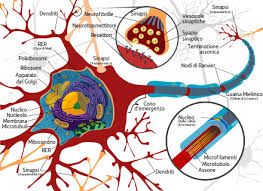
\includegraphics[scale=0.7]{neurone.jpeg}
\caption{Neurone}
\label{fig:1}
\end{figure}

Il cervello è composto da miliardi di cellule dette \emph{neuroni} (Figura \ref{fig:1}). Il neurone a sua volta è costituito da:
\begin{itemize}
\item{i \emph{dendriti}, i quali sono filamenti raggiunti dalle terminazioni di altri neuroni e che gli permettono di raccogliere informazioni grazie a processi biochimici originati dai così detti \emph{neurotrasmettitori}.}
\item{l'\emph{assone}: un lungo filamento che parte dal corpo centrale della cellula e trasmette segnali elettrici che, a loro volta, vanno ad attivare altri neuroni attraverso il rilascio di neurotrasmettitori.}
\end{itemize}

Quando e come il neurone trasmetta il segnale di attivazione dipende dal particolare modello fisiologico che si voglia adottare. Solitamente si considera un \emph{threshold}, superato il quale, l'assone viene depolarizzato e la differenza di potenziale provoca il passaggio di una corrente. Un diverso modello prende in considerazione non tanto la potenza dello stimolo quanto il loro numero. 
Questa struttura a network offre ottime prestazioni. Per un confronto con una CPU classica alleghiamo la seguente tabella:

\begin{figure}
\centering
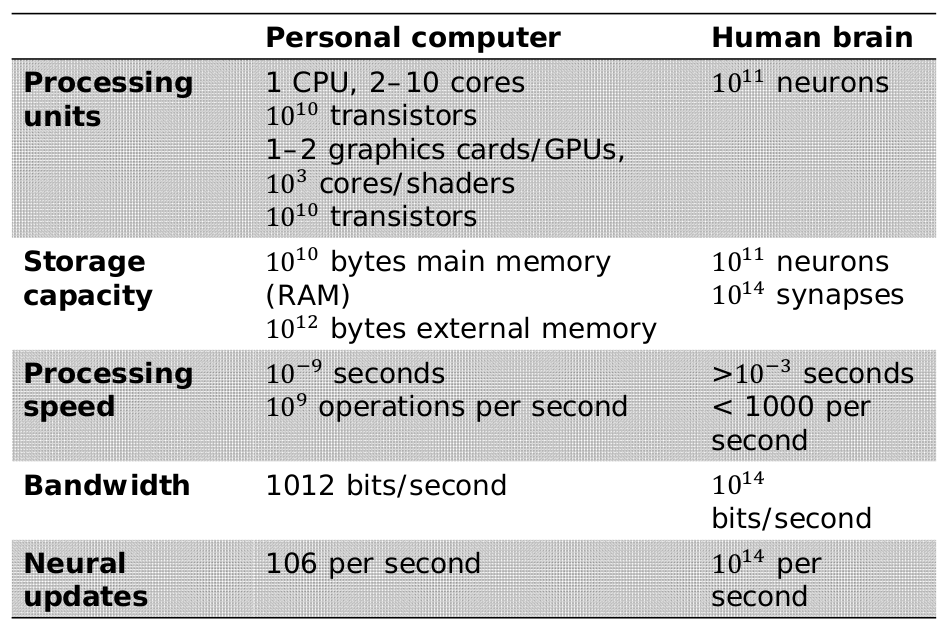
\includegraphics[scale=0.3]{cpuvshuman.png}
\end{figure}

\newpage

I vantaggi delle reti neurali sono:

\begin{enumerate}
\item{Alta velocità di calcolo, grazie al parallelismo.}
\item{Tolleranza ai guasti: la rete rimane funzionale anche quando molti neuroni smettono di funzionare.}
\item{La performance degrada in modo lineare con il numero di neuroni danneggiati.}
\item{Ottimo per l'apprendimento induttivo.}
\end{enumerate}

\subsection{Threshold logic unit}

Per implementare una rete neurale artificiale occorre trovare un analogo del neurone naturale. Tale compito è svolto dalle \emph{threshold logic unit}, nel seguito TLU. Una TLU è costituita da $n$ variabili di input $x_1 \dots x_n$ e un output $y$. Ad ogni unità viene assegnato un \emph{threshold} $\theta$ e ad ogni variabile di input un peso $w_i$ dove $i \in \{1, \dots ,n\}$ che rappresenta la rilevanza ai fine della computazione di quel particolare input.
L'output della TLU viene calcolato secondo la seguente formula:

\begin{equation}
y =  \begin{cases}
    1 & \text{se } \sum w_ix_i \geq \theta \\
    0 & \text{altrimenti} 
   \end{cases}
\end{equation}

Attraverso questo semplice meccanismo possiamo simulare alcune funzioni booleane. Se volessimo computare l'AND logico tra due input $x_1$ e $x_2$ basta assegnare valori ai pesi e al threshold in modo che soddisfino il seguente sistema di disequazioni:

\begin{equation}
	\begin{cases}
    w_1 + w_2 \geq \theta \\
    w_1 < \theta\\
    w_2 < \theta
   \end{cases}
\end{equation}

Risulta evidente che l'unica circostanza in cui l'output della TLU verrà posto ad 1 sarà quando entrambi gli input si trovano a 1. Inoltre, si noti che esistono varie scelte possibili di pesi e threshold che verificano le diseguaglianze.

\subsection{Interpretazione geometrica}

La condizione che calcola l'output della TLU somiglia molto da vicino all'equazione di un iperpiano (ovvero, un piano in $n$ dimensioni):

\begin{equation}
	 \sum w_ix_i + \theta = 0 
\end{equation}

Se pensiamo al caso precedente dell'AND logico e consideriamo i valori di input come coordinate in uno spazio bidimensionale, possiamo vedere che la retta definita da $x_1w_1 + x_2w_2 + \theta = 0$ corrisponde al confine che separa quelle combinazioni di valori che restituiscono come output 1 e quelle che, invece, restituiscono 0 (vedi Figura 2). \\
Da quanto detto, tuttavia, si può dedurre che una singola TLU potrà computare solo funzioni \emph{linearmente separabili}, ovvero funzioni in cui le coordinate associate agli input che restituiscono 1 possono essere separate da quelle che restituiscono 0 da una funzione lineare (punto, retta, piano o iperpiano a seconda della dimensione). 

\begin{figure}
\centering
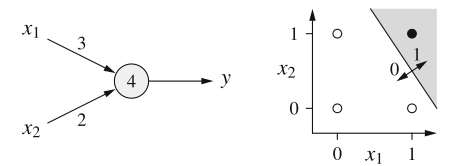
\includegraphics[scale=0.5]{geometria.png}
\caption{Rappresentazione geometrica della TLU per $x_1 \land x_2$}
\label{fig:2}
\end{figure}

\begin{definition}
Un insieme di punti $X$ in uno spazio euclideo si dice \emph{convesso} se e solo se non è vuoto, è connesso e ogni coppia di punti può essere congiunta da un segmento.
\end{definition}
\begin{definition}
Un \emph{guscio convesso} di un insieme di punti $X$ in uno spazio euclideo è il più piccolo insieme convesso che contiene $X$.
\end{definition}
\begin{theorem}
Due insiemi di punti $X$ e $Y$ si dicono linearmente separabili se e solo se i loro gusci convessi sono tra loro disgiunti.
\end{theorem}

Questo significa che già all'interno delle funzioni booleane ne esistono alcune che non possono essere simulate da una TLU. Come, per esempio, la doppia implicazione. Sebbene solo due funzioni booleane a due argomenti non siano linearmente indipendenti, al crescere degli argomenti il numero di funzioni che sono linearmente indipendenti diminuisce rapidamente. Per un numeri di argomenti arbitrariamente grande, una singola TLU non può calcolare "quasi" nessuna funzione.

\begin{figure}
\centering
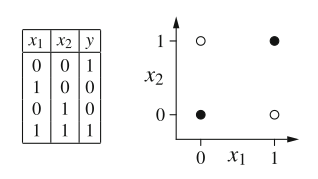
\includegraphics[scale=0.5]{doppiaimplicazione.png}
\caption{La doppia implicazione non è linearmente separabile}
\label{fig:3}
\end{figure}

Il problema può essere ovviato attraverso la costruzione di network di TLU più complessi. Come esempio consideriamo il network che simula la doppia implicazione (vedi figura \ref{fig:4}).

\begin{figure}
\centering
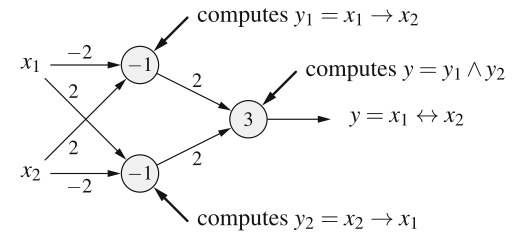
\includegraphics[scale=0.5]{netTLU.png}
\caption{network di TLU che simula la doppia implicazione}
\label{fig:4}
\end{figure}

\subsection{Training delle TLU}

L'interpretazione geometrica ci da una intuizione su come costruire una TLU avente 2 o 3 input, ma non è un metodo scalabile, nè automatizzato. Come far evolvere una TLU affinchè converga in modo autonomo ad una soluzione?
Un algoritmo che ci permette di automatizzare il processo è il seguente:

\begin{enumerate}
\item{Inizializzare i pesi e il threshold con valori randomici.}
\item{Determinare l'errore nell'output per un insieme di controlli. L'errore viene calcolato come una funzione dei pesi e del threshold $e(w_1,\dots,w_n,\theta)$.}
\item{Aggiornare i pesi e il threshold per correggere l'errore.}
\item{Iterare finchè l'errore si annulla.}
\end{enumerate}

Mostriamo il comportamento dell'algoritmo nel caso più semplice, in cui abbiamo un threshold ed un unico input (quindi, un unico peso associato). Poniamo che si voglia allenare il nostro neurone a calcolare la negazione booleana. Sia $x$ l'input, $w$ il peso associato e $\theta$ il threshold, allora l'output $y$ sarà definito come:

\begin{equation}
	y = \begin{cases}
    1 & \text{se } 0w = 0 \geq \theta \\
    0 & \text{se } 1w = w \geq \theta
   \end{cases}
\end{equation} 

Calcoliamo la funzione errore al variare di $w$ e $\theta$. Nel caso che $x = 0$ l'errore sarà 0 per un $\theta$ negativo e 1 per un $\theta$ negativo. Il peso non avrà alcuna influenza perchè viene annullato nella moltiplicazione con l'input. Quando, invece, $x = 1$, avremo che la funzione dipenderà da entrambi i parametri (vedi Figura \ref{fig:5}).

\begin{figure}
\centering
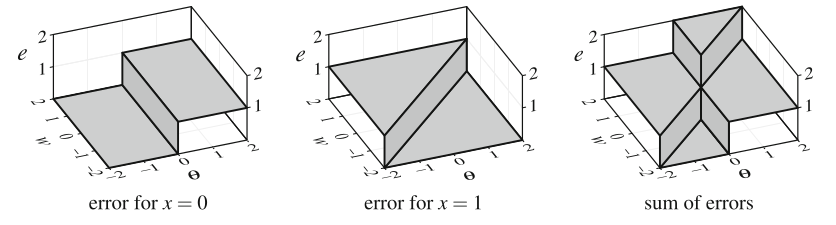
\includegraphics[scale=0.5]{error1.png}
\caption{funzione di errore per la negazione booleana}
\label{fig:5}
\end{figure}

La funzione di errore così calcolata non può essere usata direttamente nella nostra computazione perchè è composta da plateau e, quindi, non è ovunque derivabile. La soluzione è quella di calcolare la funzione di errore in modo tale che ci offra una misura di "quanto sbagliata" sia la relazione tra pesi e threshold. Otterremo così una funzione di errore che, seppur ancora non differenziabile, (vedi Figura \ref{fig:6}) lo sia localmente nei punti in cui l'errore si discosta da $0$. Ciò che faremo per correggere l'errore, dunque, sarà discendere verso l'area dove la funzione di errore si annulla. Questo è possibile esattamente perché abbiamo costruito una funzione derivabile nei punti in cui ci interessa, e cioè possiamo sempre calcolare la direzione migliore da prendere perchè si "scenda".
Ci sono due modi di immaginare il processo di allenamento del neurone:

\begin{itemize}
\item{\emph{Online learning}: dove correggiamo l'errore individualmente per ogni scelta dell'input.}
\item{\emph{Batch learning}: dove prendiamo in considerazione l'errore cumulato su una sequenza di input prima di applicare le correzioni.}
\end{itemize}

\begin{figure}
\centering
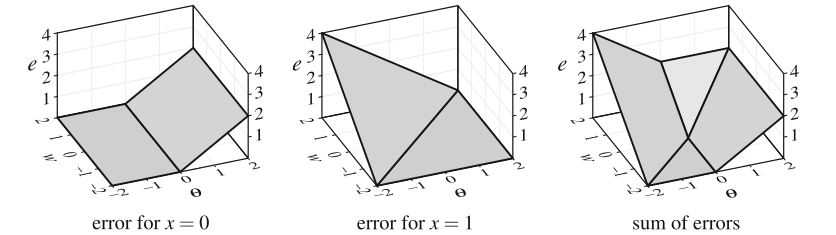
\includegraphics[scale=0.5]{error2.png}
\caption{funzione di errore differenziabile}
\label{fig:6}
\end{figure}

Definiamo di seguito la \emph{delta rule} o \emph{procedura di Widrow-Hoff} per allenare le TLU:

\begin{definition}
Sia $\vv$ = ($x_1, \dots, x_n$) il vettore di input di una TLU, \emph{o} l'output aspettato e \emph{y} il valore attuale. Se \emph{o} = \emph{y}, abbiamo finito. Al contrario, per ridurre l'errore computeremo nuovi valori per il threshold e i pesi nel seguente modo:
$$
\theta^{(new)} = \theta^{(old)} + \Delta\theta \text{ con } \Delta\theta = -\eta(\emph{o} - \emph{y})
$$
$$
\forall i \in \{1, \dots, n\}:w_i^{(new)} = w_i^{(old)} + \Delta w_i \text{ con } \Delta w_i = \eta(\emph{o} - \emph{y})x_i
$$
dove $\eta$ è il \emph{learning rate}. Più è alto, più i cambiamenti sui pesi e sui threshold sono drastici.

\end{definition}

Abbiamo visto prima, tuttavia, che non tutte le funzioni possono essere computate. Per le funzioni linearmente separabili esiste un teorema che ci garantisce che applicando la \emph{delta rule} l'algoritmo converga ad una soluzione.

\begin{theorem}
Sia $L = \{(\vv_1,\emph{o}_1), \dots, (\vv_n,\emph{o}_n)\}$ una sequenza di pattern di allenamento per la TLU, dove $\vv_i$ sono i vettori di input e $\emph{o}_i$ l'output atteso. 
Siano inoltre $L_0 = \{(\vv,\emph{o}) \in L | \emph{o} = 0\}$ e $L_1 = \{(\vv,\emph{o}) \in L | \emph{o} = 1\}$ rispettivamente gli insiemi delle coppie di pattern che hanno come output atteso 0 e quelle che hanno come pattern atteso 1. Se $L_0$ e $L_1$ sono linearmente separabili, allora esiste un $\ww$ vettore di pesi e un $\theta$ threshold t.c.:
$$
\forall (\vv,0) \in L_0: \ww\vv < \theta 
$$
$$
\forall (\vv,1) \in L_1: \ww\vv \geq \theta
$$
\end{theorem}

\begin{remark}
Negli esempi precedenti abbiamo codificato il valore booleano \emph{falso} come 0 e \emph{vero} come 1. Questa scelta non è felice perchè ha lo svantaggio che, nel caso di \emph{falso}, i pesi corrispondenti perchè la formula contiene l'input come fattore. Per evitare il problema si ricorre in letteratura ad una diversa codifica chiamata \emph{ADALINE} (ADAptive LINear Element), dove \emph{falso} viene ad assumere il valore $-1$ e il \emph{vero} $1$.
\end{remark}

Notiamo che questa procedura di allenamento vale solo per le singole TLU, ma abbiamo prima visto che le TLU possono computare solo funzioni linearmente separabili. Sebbene questo inconveniente si possa evitare prendendo in esame \emph{network} di TLU, questa procedura non si estende naturalmente a quel caso.

\section{Sistemi fuzzy}

\section{Algoritmi evolutivi}


\end{document}